\documentclass{article}
% Fall 2026 course Project template (the class file itself supplies the course footer).
\usepackage[final]{corl_2023}
\usepackage[T1]{fontenc}
\usepackage[utf8]{inputenc}
\usepackage{amsmath,amssymb}
\usepackage{enumitem,graphicx}
\usepackage{tikz}
\usetikzlibrary{positioning,arrows.meta,fit,backgrounds}
\usepackage{placeins}
\setlist{itemsep=0pt,topsep=2pt}

\newcommand{\src}{\mathcal{S}}
\newcommand{\tgt}{\mathcal{T}}

\title{{\Large Mind the Touch Gap: Real-to-Sim Contact\\Alignment for Dexterous Pen Spinning}}
\hypersetup{pdftitle={Mind the Touch Gap: Real-to-Sim Contact Alignment for Dexterous Pen Spinning},pdfauthor={Xinyao Li, Wen-Han Hsieh, Seungjae Baek, Shuai Zhou, Yuan Li, Yusu Fang},pdfsubject={16-831 Fall 2026 Course Project Proposal}}
\author{
  Xinyao Li\\{\normalfont\small xinyaol2}\\{\normalfont\small\texttt{xinyaol2@andrew.cmu.edu}}
  \And
  Wen-Han Hsieh\\{\normalfont\small wenhanh}\\{\normalfont\small\texttt{wenhanh@andrew.cmu.edu}}
  \And
  Seungjae Baek\\{\normalfont\small seungjab}\\{\normalfont\small\texttt{seungjab@andrew.cmu.edu}}
  \AND
  Shuai Zhou\\{\normalfont\small shuaizho}\\{\normalfont\small\texttt{shuaizho@andrew.cmu.edu}}
  \And
  Yuan Li\\{\normalfont\small yuanli5}\\{\normalfont\small\texttt{yuanli5@andrew.cmu.edu}}
  \And
  Yusu Fang\\{\normalfont\small yusuf}\\{\normalfont\small\texttt{yusuf@andrew.cmu.edu}}
}

\begin{document}
\maketitle

\begin{abstract}
Pen spinning is fast and contact-rich, making simulation transfer difficult. PenSpin~\citep{wang2024penspin} fine-tuned a proprioceptive student on successful hardware replays. We ask whether a small replay budget can also improve the contact observations used during simulator training. Using Isaac Gym~\citep{makoviychuk2021isaac} and Project SuperDex~\citep{superdex2026}, we will learn a source-to-target contact mapper, re-distill a contact-aware student, and compare it with proprio-only, raw-contact, randomized-contact, calibrated-contact, and target-fine-tuning baselines. This controlled sim-to-sim study evaluates whether better contact observations improve cross-simulator transfer.
\end{abstract}
\keywords{Dexterous manipulation, contact alignment, sim-to-sim transfer}

% ===========================================================================
\section{Introduction}

Reinforcement learning in simulation has made dexterous in-hand skills possible without collecting large numbers of difficult demonstrations~\citep{qi2022hora,openai2020dexterous,qi2023general}. Pen spinning is an especially demanding case: the pen must pass through rapid, repeated contacts, and a small error in timing can end a rotation. PenSpin~\citep{wang2024penspin} trained a privileged oracle in simulation and distilled a proprioceptive student, but transferring the student directly to hardware remained difficult. Its solution was to replay the oracle's actions open-loop on the hand, retain successful trajectories, and fine-tune the student on those demonstrations.

This result shows the value of even a small amount of target experience, while leaving open how that experience might improve subsequent training in simulation. Prior work has used real experience to adapt simulation parameters~\citep{chebotar2019closing,he2025asap,ramos2019bayessim}, including recent tactile calibration through trajectory replay~\citep{real2sim2real2026}. For pen spinning, the contact signal is a natural place to investigate: it changes rapidly during a spin and may differ across simulators even when the same actions are applied. We study this question in a controlled sim-to-sim setting, training in Isaac Gym~\citep{makoviychuk2021isaac} and evaluating in Project SuperDex~\citep{superdex2026}. SuperDex gives us contact labels and repeatable evaluations across friction and compliance settings.

The replay data may also reveal how contact readings differ between Isaac Gym and SuperDex. We will replay oracle actions in both simulators, train a mapper on the resulting contact pairs, and use its predictions to distill a contact-aware student in Isaac Gym. This extends PenSpin's proprioceptive student with link-level contact. We will compare the student's performance in SuperDex with raw contact, proprioception alone, and PenSpin-style target fine-tuning across matched replay budgets. Contact prediction and replay-state drift will help interpret the transfer results.

% ===========================================================================
\section{Plan}

We will reproduce PenSpin's oracle and student in Isaac Gym and build a matching Allegro hand and pen task in SuperDex. A small replay test will check the control and contact interfaces before data collection. We will then replay oracle actions from matched initial states in both simulators and train a temporal network to predict SuperDex link contact from Isaac Gym contact, joint states, and preceding actions. Its predictions will be used to distill a contact-aware student in Isaac Gym, which will be tested using SuperDex's own contact readings (Figure~\ref{fig:pipeline}).

We will compare aligned contact with proprioception alone, raw contact, contact randomization, simple threshold-and-delay calibration, and PenSpin-style target fine-tuning. Tests will use the same target objects and initial states across replay budgets and friction/compliance settings. We will report rotations, success, time to drop, contact F1, and replay-state drift. Target-data budgets count every replay attempt; we will also report the number of successful demonstrations available for fine-tuning.

\begin{figure}[htbp]
\centering
% Pipeline figure (TikZ). Included from main.tex via % Pipeline figure (TikZ). Included from main.tex via % Pipeline figure (TikZ). Included from main.tex via \input{figures/pipeline}.
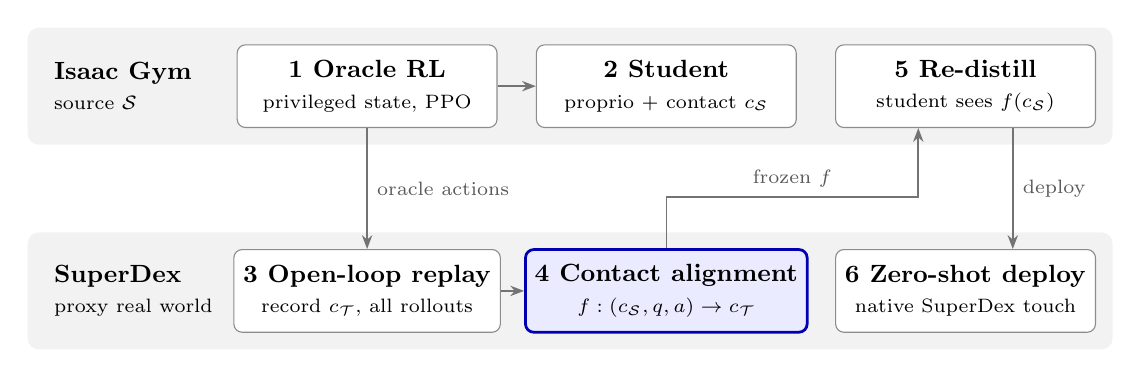
\begin{tikzpicture}[
    font=\small,
    stage/.style={draw=black!45, rounded corners=3pt, minimum width=3.3cm,
                  minimum height=1.05cm, align=center, fill=white},
    ours/.style={stage, draw=blue!70!black, line width=1pt, fill=blue!8},
    arr/.style={-{Stealth[length=5pt]}, draw=black!55, line width=0.6pt},
    lbl/.style={font=\scriptsize, text=black!65},
    lane/.style={fill=black!5, rounded corners=4pt, inner sep=6pt},
    lanename/.style={align=left, anchor=west},
  ]
  % Source row (Isaac Gym)
  \node[stage] (oracle) at (0,0)     {\textbf{1 Oracle RL}\\{\scriptsize privileged state, PPO}};
  \node[stage] (student) at (3.8,0)  {\textbf{2 Student}\\{\scriptsize proprio + contact $c_\mathcal{S}$}};
  \node[stage] (redist) at (7.6,0)   {\textbf{5 Re-distill}\\{\scriptsize student sees $f(c_\mathcal{S})$}};
  % Target row (SuperDex)
  \node[stage] (replay) at (0,-2.6)  {\textbf{3 Open-loop replay}\\{\scriptsize record $c_\mathcal{T}$, all rollouts}};
  \node[ours]  (align) at (3.8,-2.6) {\textbf{4 Contact alignment}\\{\scriptsize $f: (c_\mathcal{S}, q, a) \rightarrow c_\mathcal{T}$}};
  \node[stage] (deploy) at (7.6,-2.6){\textbf{6 Zero-shot deploy}\\{\scriptsize native SuperDex touch}};

  % Lane labels
  \node[lanename] (srcname) at (-4.1,0)   {\textbf{Isaac Gym}\\{\scriptsize source $\mathcal{S}$}};
  \node[lanename] (tgtname) at (-4.1,-2.6){\textbf{SuperDex}\\{\scriptsize proxy real world}};

  % Lane backgrounds
  \begin{scope}[on background layer]
    \node[lane, fit=(srcname)(oracle)(redist)] {};
    \node[lane, fit=(tgtname)(replay)(deploy)] {};
  \end{scope}

  % Connectors
  \draw[arr] (oracle) -- (student);
  \draw[arr] (oracle) -- node[lbl, right] {oracle actions} (replay);
  \draw[arr] (replay) -- (align);
  \draw[arr] (align.north) -- ++(0,0.65) -| node[lbl, pos=0.25, above] {frozen $f$} ([xshift=-0.6cm]redist.south);
  \draw[arr] ([xshift=0.6cm]redist.south) -- node[lbl, right] {deploy} ([xshift=0.6cm]deploy.north);
\end{tikzpicture}
.
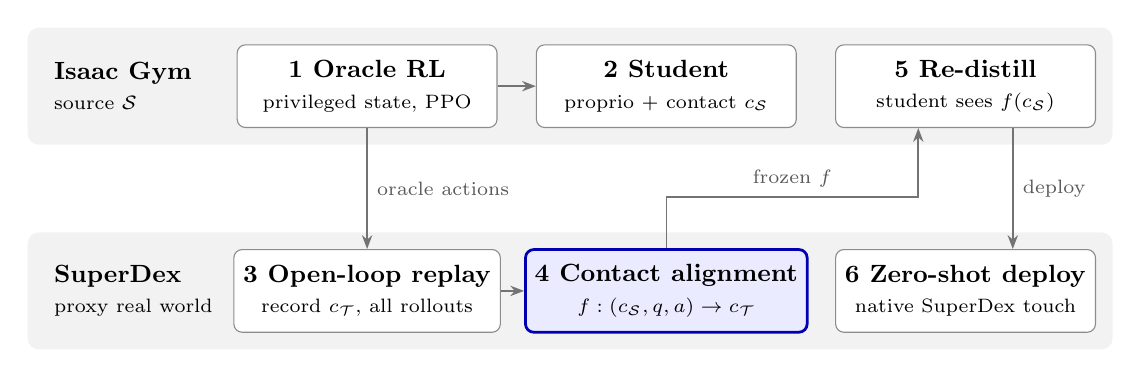
\begin{tikzpicture}[
    font=\small,
    stage/.style={draw=black!45, rounded corners=3pt, minimum width=3.3cm,
                  minimum height=1.05cm, align=center, fill=white},
    ours/.style={stage, draw=blue!70!black, line width=1pt, fill=blue!8},
    arr/.style={-{Stealth[length=5pt]}, draw=black!55, line width=0.6pt},
    lbl/.style={font=\scriptsize, text=black!65},
    lane/.style={fill=black!5, rounded corners=4pt, inner sep=6pt},
    lanename/.style={align=left, anchor=west},
  ]
  % Source row (Isaac Gym)
  \node[stage] (oracle) at (0,0)     {\textbf{1 Oracle RL}\\{\scriptsize privileged state, PPO}};
  \node[stage] (student) at (3.8,0)  {\textbf{2 Student}\\{\scriptsize proprio + contact $c_\mathcal{S}$}};
  \node[stage] (redist) at (7.6,0)   {\textbf{5 Re-distill}\\{\scriptsize student sees $f(c_\mathcal{S})$}};
  % Target row (SuperDex)
  \node[stage] (replay) at (0,-2.6)  {\textbf{3 Open-loop replay}\\{\scriptsize record $c_\mathcal{T}$, all rollouts}};
  \node[ours]  (align) at (3.8,-2.6) {\textbf{4 Contact alignment}\\{\scriptsize $f: (c_\mathcal{S}, q, a) \rightarrow c_\mathcal{T}$}};
  \node[stage] (deploy) at (7.6,-2.6){\textbf{6 Zero-shot deploy}\\{\scriptsize native SuperDex touch}};

  % Lane labels
  \node[lanename] (srcname) at (-4.1,0)   {\textbf{Isaac Gym}\\{\scriptsize source $\mathcal{S}$}};
  \node[lanename] (tgtname) at (-4.1,-2.6){\textbf{SuperDex}\\{\scriptsize proxy real world}};

  % Lane backgrounds
  \begin{scope}[on background layer]
    \node[lane, fit=(srcname)(oracle)(redist)] {};
    \node[lane, fit=(tgtname)(replay)(deploy)] {};
  \end{scope}

  % Connectors
  \draw[arr] (oracle) -- (student);
  \draw[arr] (oracle) -- node[lbl, right] {oracle actions} (replay);
  \draw[arr] (replay) -- (align);
  \draw[arr] (align.north) -- ++(0,0.65) -| node[lbl, pos=0.25, above] {frozen $f$} ([xshift=-0.6cm]redist.south);
  \draw[arr] ([xshift=0.6cm]redist.south) -- node[lbl, right] {deploy} ([xshift=0.6cm]deploy.north);
\end{tikzpicture}
.
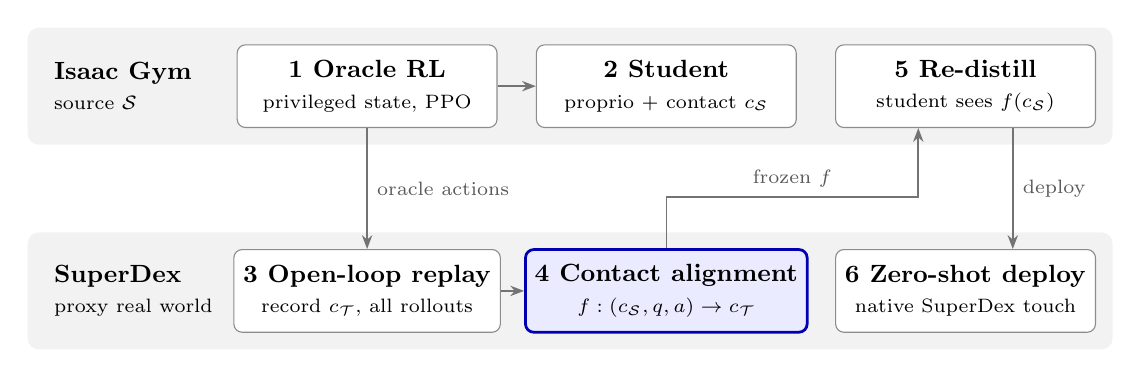
\begin{tikzpicture}[
    font=\small,
    stage/.style={draw=black!45, rounded corners=3pt, minimum width=3.3cm,
                  minimum height=1.05cm, align=center, fill=white},
    ours/.style={stage, draw=blue!70!black, line width=1pt, fill=blue!8},
    arr/.style={-{Stealth[length=5pt]}, draw=black!55, line width=0.6pt},
    lbl/.style={font=\scriptsize, text=black!65},
    lane/.style={fill=black!5, rounded corners=4pt, inner sep=6pt},
    lanename/.style={align=left, anchor=west},
  ]
  % Source row (Isaac Gym)
  \node[stage] (oracle) at (0,0)     {\textbf{1 Oracle RL}\\{\scriptsize privileged state, PPO}};
  \node[stage] (student) at (3.8,0)  {\textbf{2 Student}\\{\scriptsize proprio + contact $c_\mathcal{S}$}};
  \node[stage] (redist) at (7.6,0)   {\textbf{5 Re-distill}\\{\scriptsize student sees $f(c_\mathcal{S})$}};
  % Target row (SuperDex)
  \node[stage] (replay) at (0,-2.6)  {\textbf{3 Open-loop replay}\\{\scriptsize record $c_\mathcal{T}$, all rollouts}};
  \node[ours]  (align) at (3.8,-2.6) {\textbf{4 Contact alignment}\\{\scriptsize $f: (c_\mathcal{S}, q, a) \rightarrow c_\mathcal{T}$}};
  \node[stage] (deploy) at (7.6,-2.6){\textbf{6 Zero-shot deploy}\\{\scriptsize native SuperDex touch}};

  % Lane labels
  \node[lanename] (srcname) at (-4.1,0)   {\textbf{Isaac Gym}\\{\scriptsize source $\mathcal{S}$}};
  \node[lanename] (tgtname) at (-4.1,-2.6){\textbf{SuperDex}\\{\scriptsize proxy real world}};

  % Lane backgrounds
  \begin{scope}[on background layer]
    \node[lane, fit=(srcname)(oracle)(redist)] {};
    \node[lane, fit=(tgtname)(replay)(deploy)] {};
  \end{scope}

  % Connectors
  \draw[arr] (oracle) -- (student);
  \draw[arr] (oracle) -- node[lbl, right] {oracle actions} (replay);
  \draw[arr] (replay) -- (align);
  \draw[arr] (align.north) -- ++(0,0.65) -| node[lbl, pos=0.25, above] {frozen $f$} ([xshift=-0.6cm]redist.south);
  \draw[arr] ([xshift=0.6cm]redist.south) -- node[lbl, right] {deploy} ([xshift=0.6cm]deploy.north);
\end{tikzpicture}

\caption{Proposed training and evaluation pipeline. The target simulator provides paired contact labels for the mapper and native contact for the final policy test.}
\label{fig:pipeline}
\end{figure}
\FloatBarrier

\begin{itemize}[leftmargin=*]
  \item \textbf{10/13--10/30:} Reproduce PenSpin and complete a small Allegro/pen/contact replay test in SuperDex.
  \item \textbf{10/31--11/13:} Collect paired replays, train the contact mapper, and re-distill the student.
  \item \textbf{11/14--12/04:} Compare baselines at 10, 25, 50, and 100 replay attempts; measure rotations, drop time, success, contact F1, and state drift.
  \item \textbf{12/05--12/11:} Analyze results and prepare the final report and presentation.
\end{itemize}

If needed, we will validate the mapper first on a simpler in-hand rotation task~\citep{qi2022hora}.

\acknowledgments{ChatGPT assisted with editorial revision and LaTeX formatting.}
\bibliography{refs}
\end{document}

